\begin{figure}[H]
    \centering
    \begin{algorithm}[H]
    \caption{Algoritmo para comprimir en \texttt{RLE} con modo literal (Umbral $3$)}
    \begin{algorithmic}[1]
    \Procedure{comprimir}{$S$} \Comment{Cadena de símbolos $S$}
    \State $N \gets longitud(S)$
    \State $0 \gets []$ \Comment{Cadena de salida comprimida}
    \State $p \gets 0$
    \While{not $EOF$}
        \State $i \gets 1$
        \State $q \gets p + 1$
        \Comment{Fase 1: Contar la secuencia}
        \While{$q < N \text{ y } S[q] = S[p] \text{ y } i < 255$} \Comment{Máximo conteo en 1 byte}
            \State $i \gets i + 1$
            \State $q \gets q + 1$
        \EndWhile
        
        \Comment{Fase 2: Aplicar el umbral y codificar}
        \If{$i \geq 3$}
            \Comment{Guardar como tupla RLE: $\langle \texttt{FLAG\_RLE}, i, S_{p} \rangle$}
            \State $O \gets O \ \| \ \texttt{FLAG\_RLE} \ \| \ i \ \| \ S[p]$
        \Else
            \Comment{Guardar como secuencia literal: $S[p]$ se repite $i$ veces}
            \For{$k \gets 0 \text{ hasta } i - 1$}
                \State $O \gets O \ \| \ S[p]$
            \EndFor
        \EndIf
        
        \State $p \gets p + i$ \Comment{Mover el apuntador principal al inicio de la siguiente secuencia}
    \EndWhile
    \State \textbf{Salida:} $0$
    \EndProcedure
    \end{algorithmic}
    \end{algorithm}
    \caption{Algoritmo secuencial para comprimir}
    \label{anexo:codigo.1}
\end{figure}

\begin{figure}[H] 
    \centering 
    \begin{algorithm}[H] 
        \caption{Algoritmo para Descomprimir en \texttt{RLE} (Modo Extendido)} 
        \begin{algorithmic}[1] 
            \Procedure{descomprimir}{C} \Comment{Cadena de símbolos comprimidos C} 
            \State $N \gets longitud(C)$ 
            \State $0 \gets []$ \Comment{Cadena de salida descomprimida}
            \State $p \gets 0$

            \While{$p < N_C$}
                \State $S \gets C[p]$ \Comment{Leer el símbolo actual (byte de control o literal)}
                
                \If{$S = \texttt{FLAG\_RLE}$}
                    \If{$p + 2 \geq N_C$} 
                        \State $break$ \Comment{Error: Buffer incompleto} 
                    \EndIf
                    
                    \State $i \gets C[p+1]$ \Comment{Leer el conteo (longitud)}
                    \State $V \gets C[p+2]$ \Comment{Leer el valor del símbolo}
                    
                    \For{$k \gets 1 \text{ hasta } i$}
                        \State $O \gets O \ \| \ V$ \Comment{Escribir el valor $V$ el número de veces $i$}
                    \EndFor
                    \State $p \gets p + 3$ \Comment{Avanzar el apuntador 3 posiciones (FLAG, Conteo, Valor)}
                    
                \ElsIf{$S = \texttt{FLAG\_LITERAL}$} \Comment{Símbolo $FLAG$ escapado}
                    \If{$p + 1 \geq N_C$} 
                        \State $break$ \Comment{Error: Buffer incompleto} 
                    \EndIf
                    
                    \State $V \gets C[p+1]$ \Comment{Leer el siguiente byte (que es un FLAG real)}
                    \State $O \gets O \ \| \ V$ \Comment{Escribir el byte escapado}
                    \State $p \gets p + 2$ \Comment{Avanzar 2 posiciones (FLAG\_LITERAL, Valor)}
                    
                \Else \Comment{Símbolo sin repetición}
                    \State $O \gets O \ \| \ S$ \Comment{Escribir el símbolo literal actual $S$}
                    \State $p \gets p + 1$ \Comment{Avanzar 1 posición}
                \EndIf
            \EndWhile
        \State \textbf{Salida:} $O$
        \EndProcedure
        \end{algorithmic}
    \end{algorithm}
        \caption{Algoritmo secuencial para descomprimir}
    \label{anexo:codigo.2}
\end{figure}

\begin{figure}[H] 
    \centering 
    \begin{algorithm}[H] \caption{Algoritmo para comprimir en \texttt{RLE} en paralelo} 
        \begin{algorithmic}[1]
            \Procedure{comprimir\_paralelo}{S,N} 
                \Comment{$S$ entrada y $N$ número de procesos} \\
                \Comment{Lógica del Coordinador (Pre-procesamiento)}
                \State $Global\_Size \gets longitud(S)$ 
                \For{$id \gets 0 \ldots N - 1$} 
                    \State $\text{OffsetStart}$
                    \State $SizeChunk \gets calculate\_chunk(id,Global\_Size,S) $
                    \State $Chunkid \gets S[OffsetStart \ldots OffsetStart + SizeChunk +1]$ 
                    
                    \Comment{Incluye 1 byte de frontera} 
                    \State $\text{Enviar}(Chunkid) \text{ a } N\_id$
                \EndFor 
                \State $Sincronizar()$

                \Comment{Lógica del Trabajador}
                \State $\text{Input}_{\text{T}} \gets \textbf{Recibir}(\text{Chunk}_{\text{id}})$
                \State $\text{Input}_{\text{Main}} \gets \text{Input}_{\text{T}}[\text{datos principales}]$
                \State $\text{Byte}_{\text{Next}} \gets \text{Input}_{\text{T}}[\text{byte de frontera}]$
                \State $\text{Output}_{\text{local}} \gets \text{Comprimir\_Secuencial}(\text{Input}_{\text{Main}})$ 
                \Comment{Usa RLE Extendido}
                
                \\
                \Comment{Corrección de Fronteras (Comunicación/Sincronización)}
                \If{$id < N - 1$}
                    \State $\text{Enviar\_Front}(\text{Output}_{\text{local}}.\text{último\_bloque}) \text{ a } \text{Trabajador}_{\text{id}+1}$
                    \State $\text{Recibir\_Front}(\text{Señal}_{\text{Fus}}) \text{ de } \text{Trabajador}_{\text{id}+1}$
                    \If{$\text{Señal}_{\text{Fus}} = \text{FUSIONADO}$}
                        \State $\text{Output}_{\text{local}}.\text{Eliminar\_último\_bloque}()$
                    \EndIf
                \EndIf
                
                \If{$id > 0$}
                    \State $\text{Recibir\_Front}(\text{Bloque}_{\text{Prev}}) \text{ de } \text{Trabajador}_{\text{id}-1}$
                    \State $\text{Intentar\_Fusion}(\text{Output}_{\text{local}}.\text{primero}, \text{Bloque}_{\text{Prev}})$
                    \State $\text{Enviar\_Front}(\text{Señal}_{\text{Fus}}) \text{ a } \text{Trabajador}_{\text{id}-1}$
                \EndIf
                
                \State $\textbf{Enviar}(\text{Output}_{\text{local}}) \text{ al Coordinador}$
                \State $\textbf{Sincronizar}()$
                
                \Comment{Lógica del Coordinador (Post-procesamiento)}
                \State $\text{Recibir\_Buffers}(\text{Todos los trabajadores})$
                \State $\text{Len}_{\text{Acumulada}} \gets \text{Calcular\_Suma\_Prefijo}(\text{Longitudes\_locales})$
                \State $O_{\text{comp}} \gets \text{Concatenar}(\text{Buffers recibidos}, \text{Len}_{\text{Acumulada}})$
                \State \textbf{Salida:} $O_{\text{comp}}$
            \EndProcedure
        \end{algorithmic}
    \end{algorithm}
    \caption{Algoritmo paralelo para comprimir}
    \label{anexo:codigo.3}
\end{figure}

\begin{figure}[H] 
    \centering 
    \begin{algorithm}[H] \caption{Algoritmo para descomprimir en \texttt{RLE} en paralelo} 
        \begin{algorithmic}[1]
            \Procedure{descomprimir\_paralelo}{C,$N$}
                \Comment{$C$ entrada comprimida y $N$ número de procesos} \\
                \Comment{Lógica del Coordinador (Pre-procesamiento)}
                \State $Par_{count} \gets read\_Metadato(C)$ 
                \Comment{Número total de pares/bloques} 
                \For{$id \gets 0 \ldots N -1$} 
                    \State $Offset_{par},Size_{par} \gets Calcular\_Particion\_Pares(id,Par_{count})$ 
                    \State $Chunk_{id} \gets C[Offset_{par} \ldots Offset_{par} + Size_{par}]$ 
                    \Comment{Lectura de porción de pares}
                    \State $\text{Enviar}(Chunkid) \text{ a } N\_id$
                \EndFor 
                \State $Sincronizar()$
                \\
                \Comment{Lógica del Trabajador}
                \State $\text{Input}_{\text{T}} \gets \textbf{Recibir}(\text{Chunk}_{\text{id}})$
                \State $\text{Output}_{\text{local}} \gets \text{Descomprimir\_Secuencial}(\text{Input}_{\text{T}})$ 
                \Comment{Genera bytes sin comprimir}
                \State $\text{Len}_{\text{local}} \gets \text{longitud}(\text{Output}_{\text{local}})$
                
                \\
                \Comment{Cálculo del Offset Global (Suma Prefijo)}
                \State $\textbf{Enviar}(\text{Len}_{\text{local}}) \text{ a Concentrador}$
                \State $\textbf{Sincronizar}()$
                
                \State $\text{Recibir}(\text{Todas\_Len}_{\text{local}})$
                \State $\text{Offset}_{\text{Final}} \gets \text{Calcular\_Suma\_Prefijo}(\text{Todas\_Len}_{\text{local}})[\text{id}]$ 
                \\
                \Comment{Cada trabajador conoce dónde escribir}
                
                \State $\textbf{Escribir\_en\_Posicion\_Global}(O_{\text{descomp}}, \text{Offset}_{\text{Final}}, \text{Output}_{\text{local}})$ 
                \\
                \Comment{Escritura dispersa}
                

                \State $\textbf{Sincronizar}()$
                
                \\
                \Comment{Lógica del Coordinador (Post-procesamiento)}
                \State $\text{Finalizar\_Archivo}(O_{\text{descomp}})$
                \State \textbf{Salida:} $O_{\text{descomp}}$
            \EndProcedure
        \end{algorithmic}
    \end{algorithm}
    \caption{Algoritmo paralelo para descomprimir}
    \label{anexo:codigo.4}
\end{figure}

\sisetup{
    round-mode = places,
    round-precision = 4,
    table-format = 1.4
}

\begin{table}[h!]
    \centering
    \caption{Resultados de rendimiento para el archivo de \textbf{Alta Repetitividad} (\texttt{data\_plana.bin}).}
    \label{tab:plana}
    \begin{tabular}{
        l
        l % Procesos (2 dígitos)
        S[table-format = 1.4] % Tiempo Promedio (s)
        S[table-format = 1.2] % Speedup (1 dígito entero, 2 decimales)
    }
        \toprule
        \textbf{Archivo} & {\textbf{Procesos}} & {\textbf{Tiempo Promedio (s)}} & {\textbf{Speedup ($S$)}} \\
        \midrule
        \texttt{data\_plana.bin} & 1 & 0.1341 & 1.00 \\
        \texttt{data\_plana.bin} & 2 & 0.0929 & 1.44 \\
        \texttt{data\_plana.bin} & 4 & 0.0723 & 1.86 \\
        \texttt{data\_plana.bin} & 6 & 0.0701 & 1.91 \\
        \texttt{data\_plana.bin} & 8 & 0.0848 & 1.58 \\
        \texttt{data\_plana.bin} & 10 & 0.0892 & 1.50 \\
        \texttt{data\_plana.bin} & 16 & 0.0973 & 1.38 \\
        \bottomrule
    \end{tabular}
\end{table}

\begin{table}[h!]
    \centering
    \caption{Resultados de rendimiento para el archivo de \textbf{Media Repetitividad} (\texttt{data\_malla.bin}).}
    \label{tab:malla}
    \begin{tabular}{
        l
        l
        S[table-format = 1.4]
        S[table-format = 1.2]
    }
        \toprule
        \textbf{Archivo} & {\textbf{Procesos}} & {\textbf{Tiempo Promedio (s)}} & {\textbf{Speedup ($S$)}} \\
        \midrule
        \texttt{data\_malla.bin} & 1 & 0.5299 & 1.00 \\
        \texttt{data\_malla.bin} & 2 & 0.3366 & 1.57 \\
        \texttt{data\_malla.bin} & 4 & 0.2123 & 2.50 \\
        \texttt{data\_malla.bin} & 6 & 0.2413 & 2.20 \\
        \texttt{data\_malla.bin} & 8 & 0.2458 & 2.16 \\
        \texttt{data\_malla.bin} & 10 & 0.3061 & 1.73 \\
        \texttt{data\_malla.bin} & 16 & 0.3196 & 1.66 \\
        \bottomrule
    \end{tabular}
\end{table}

\begin{table}[h!]
    \centering
    \caption{Resultados de rendimiento para el archivo \textbf{Aleatorio} (Peor Caso) (\texttt{data\_aleatoria.bin}).}
    \label{tab:aleatoria}
    \begin{tabular}{
        l
        l
        S[table-format = 1.4]
        S[table-format = 1.2]
    }
        \toprule
        \textbf{Archivo} & {\textbf{Procesos}} & {\textbf{Tiempo Promedio (s)}} & {\textbf{Speedup ($S$)}} \\
        \midrule
        \texttt{data\_aleatoria.bin} & 1 & 0.5613 & 1.00 \\
        \texttt{data\_aleatoria.bin} & 2 & 0.3522 & 1.59 \\
        \texttt{data\_aleatoria.bin} & 4 & 0.2324 & 2.42 \\
        \texttt{data\_aleatoria.bin} & 6 & 0.2388 & 2.35 \\
        \texttt{data\_aleatoria.bin} & 8 & 0.2399 & 2.34 \\
        \texttt{data\_aleatoria.bin} & 10 & 0.3187 & 1.76 \\
        \texttt{data\_aleatoria.bin} & 16 & 0.3505 & 1.60 \\
        \bottomrule
    \end{tabular}
\end{table}

\begin{figure}[h!]
    \centering
    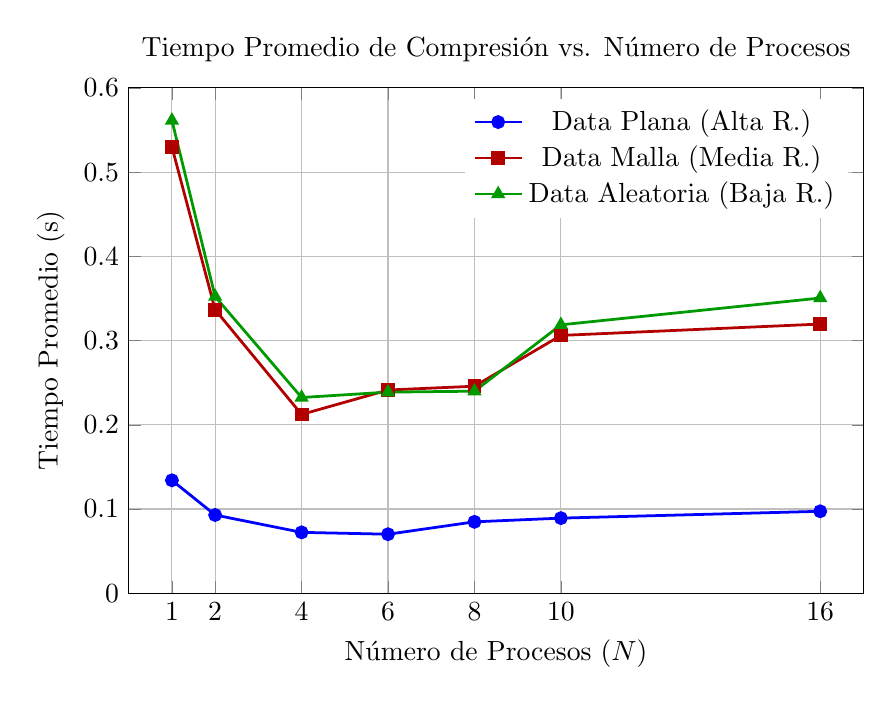
\begin{tikzpicture}
        \begin{axis}[
            % Configuración del Eje
            title={Tiempo Promedio de Compresión vs. Número de Procesos},
            xlabel={Número de Procesos ($N$)},
            ylabel={Tiempo Promedio (s)},
            xmin=0, xmax=17,
            ymin=0, ymax=0.6,
            ytick distance=0.1,
            xtick={1, 2, 4, 6, 8, 10, 16},
            grid=both, 
            legend style={
                at={(0.98,0.98)},
                anchor=north east,
                draw=none
            },
            width=0.9\textwidth,
            height=8cm,
        ]
        \addplot[
            color=blue,
            mark=*,
            line width=1pt,
        ] coordinates {
            (1, 0.1341) 
            (2, 0.0929) 
            (4, 0.0723) 
            (6, 0.0701) 
            (8, 0.0848) 
            (10, 0.0892) 
            (16, 0.0973) 
        };
        \addlegendentry{Data Plana (Alta R.)}
        \addplot[
            color=red!70!black,
            mark=square*,
            line width=1pt,
        ] coordinates {
            (1, 0.5299) 
            (2, 0.3366) 
            (4, 0.2123) 
            (6, 0.2413) 
            (8, 0.2458) 
            (10, 0.3061) 
            (16, 0.3196) 
        };
        \addlegendentry{Data Malla (Media R.)}
        \addplot[
            color=green!60!black,
            mark=triangle*,
            line width=1pt,
        ] coordinates {
            (1, 0.5613) 
            (2, 0.3522) 
            (4, 0.2324) 
            (6, 0.2388) 
            (8, 0.2399) 
            (10, 0.3187) 
            (16, 0.3505) 
        };
        \addlegendentry{Data Aleatoria (Baja R.)}
        \end{axis}
    \end{tikzpicture}
    \caption{Gráfica del tiempo de compresión promedio en función del número de procesos para los tres tipos de archivos.}
    \label{fig:tiempo_vs_procesos}
\end{figure}

\begin{figure}[h!]
    \centering
    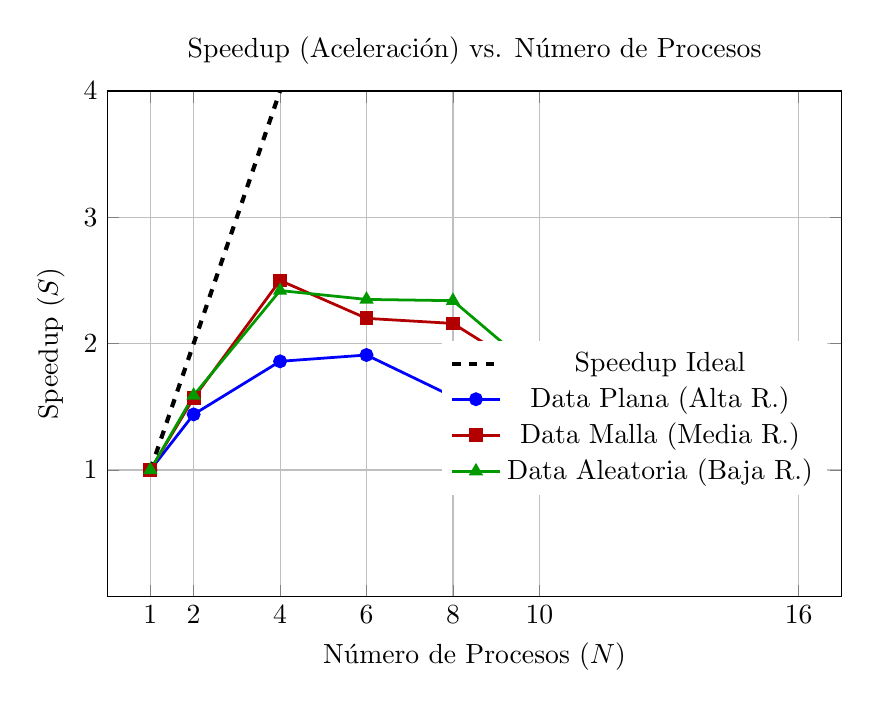
\begin{tikzpicture}
        \begin{axis}[
            % Configuración del Eje
            title={Speedup (Aceleración) vs. Número de Procesos},
            xlabel={Número de Procesos ($N$)},
            ylabel={Speedup ($S$)},
            xmin=0, xmax=17,
            ymin=0, ymax=4, % Ajuste el máximo del eje Y para incluir Speedup Ideal
            xtick={1, 2, 4, 6, 8, 10, 16},
            ytick={1, 2, 3, 4},
            grid=both, % Configuración de Leyenda
            legend style={
                at={(0.98,0.2)}, 
                anchor=south east,
                draw=none
            },
            width=0.9\textwidth,
            height=8cm,
        ]
        % Speedup IDEAL (Línea de referencia S = N)
        \addplot[
            color=black,
            dashed,
            line width=1.5pt,
        ] coordinates {
            (1, 1) (2, 2) (4, 4) (6, 6) (8, 8) (10, 10) (16, 16)
        };
        \addlegendentry{Speedup Ideal}
        % 1. Data Plana (Alta Repetitividad)
        \addplot[color=blue, mark=*, line width=1pt,] coordinates {
            (1, 1.00) (2, 1.44) (4, 1.86) (6, 1.91) (8, 1.58) (10, 1.50) (16, 1.38) 
        };
        \addlegendentry{Data Plana (Alta R.)}
        % 2. Data Malla (Media Repetitividad)
        \addplot[color=red!70!black, mark=square*, line width=1pt,] coordinates {
            (1, 1.00) (2, 1.57) (4, 2.50) (6, 2.20) (8, 2.16) (10, 1.73) (16, 1.66) 
        };
        \addlegendentry{Data Malla (Media R.)}
        % 3. Data Aleatoria (Baja Repetitividad / Peor Caso)
        \addplot[color=green!60!black, mark=triangle*, line width=1pt,] coordinates {
            (1, 1.00) (2, 1.59) (4, 2.42) (6, 2.35) (8, 2.34) (10, 1.76) (16, 1.60) 
        };
        \addlegendentry{Data Aleatoria (Baja R.)}
        \end{axis}
    \end{tikzpicture}
    \caption{Gráfica de Speedup obtenido. La aceleración ideal es la línea de referencia.}
    \label{fig:speedup_vs_procesos}
\end{figure}

\begin{figure}[h!]
    \centering
    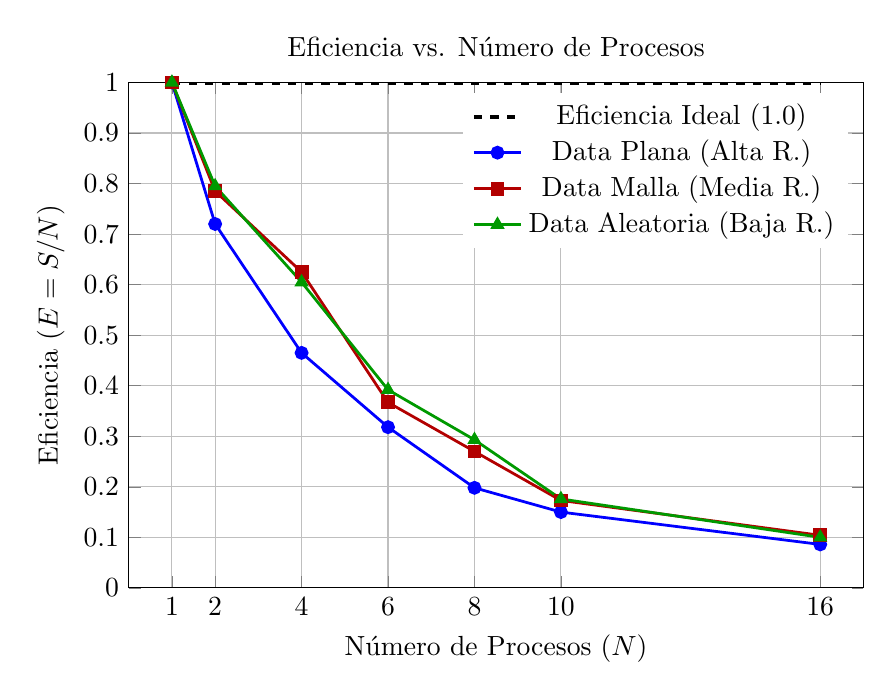
\begin{tikzpicture}
        \begin{axis}[
            % Configuración del Eje
            title={Eficiencia vs. Número de Procesos},
            xlabel={Número de Procesos ($N$)},
            ylabel={Eficiencia ($E = S/N$)},
            xmin=0, xmax=17,
            ymin=0, ymax=1.0,
            ytick distance=0.1,
            xtick={1, 2, 4, 6, 8, 10, 16},
            grid=both, 
            % Configuración de Leyenda
            legend style={
                at={(0.98,0.98)}, 
                anchor=north east,
                draw=none
            },
            width=0.9\textwidth,
            height=8cm,
        ]
        % Línea de Eficiencia 1.0 (Ideal)
        \addplot[
            color=black,
            dashed,
            line width=1.5pt,
        ] coordinates {
            (1, 1.0) (16, 1.0) 
        };
        \addlegendentry{Eficiencia Ideal (1.0)}
        % 1. Data Plana (Eficiencia = S/N)
        \addplot[color=blue, mark=*, line width=1pt,] coordinates {
            (1, 1.000) 
            (2, 0.720) % 1.44 / 2
            (4, 0.465) % 1.86 / 4
            (6, 0.318) % 1.91 / 6
            (8, 0.198) % 1.58 / 8
            (10, 0.150) % 1.50 / 10
            (16, 0.086) % 1.38 / 16
        };
        \addlegendentry{Data Plana (Alta R.)}
        % 2. Data Malla (Eficiencia = S/N)
        \addplot[color=red!70!black, mark=square*, line width=1pt,] coordinates {
            (1, 1.000) 
            (2, 0.785) % 1.57 / 2
            (4, 0.625) % 2.50 / 4
            (6, 0.367) % 2.20 / 6
            (8, 0.270) % 2.16 / 8
            (10, 0.173) % 1.73 / 10
            (16, 0.104) % 1.66 / 16
        };
        \addlegendentry{Data Malla (Media R.)}
        % 3. Data Aleatoria (Eficiencia = S/N)
        \addplot[color=green!60!black, mark=triangle*, line width=1pt,] coordinates {
            (1, 1.000) 
            (2, 0.795) % 1.59 / 2
            (4, 0.605) % 2.42 / 4
            (6, 0.392) % 2.35 / 6
            (8, 0.293) % 2.34 / 8
            (10, 0.176) % 1.76 / 10
            (16, 0.100) % 1.60 / 16
        };
        \addlegendentry{Data Aleatoria (Baja R.)}
        \end{axis}
    \end{tikzpicture}
    \caption{Gráfica de Eficiencia en función del número de procesos.}
    \label{fig:eficiencia_vs_procesos}
\end{figure}